\section*{RESULTADOS E DISCUSSÕES}

A avaliação em escala nacional ao longo do ano de 2025 integrou 4,05 milhões de registros provenientes de 7 bases governamentais, alocados em $\sim$850 MB no \textbf{\textit{Apache Druid}} em 695 segmentos compactados.

\begin{center}
\vspace{-0.10cm}
{\fontsize{16}{20}\selectfont
\begin{tabular}{llr}
\hline
\textbf{Entidade Lógica} & \textbf{Fonte Governamental} & \textbf{Registros Aprox.} \\
\hline
Fato Focos de Incêndio & INPE (BDQueimadas) & 3.335.198 \\
Fato Eventos Agrupados & Algoritmo \textbf{\textit{DBSCAN}} (Perímetros) & 147.560 \\
Hospitais e Unidades de Saúde & MS / DATASUS (CNES) & 550.882 \\
Rodovias Federais e Estaduais & MT / DNIT / BIT & 14.255 \\
Linhas e Subestações de Energia & MME / ANEEL / ONS & 2.564 \\
Municípios Brasileiros & IBGE (Malha Geodados) & 5.564 \\
Terras Indígenas Demarcadas & MJSP / FUNAI & 650 \\
\hline
\textbf{Total Analítico Consolidado} & \textbf{Armazenamento nos Nós Druid} & \textbf{4.056.673 ($\sim$850 MB)} \\
\hline
\end{tabular}
}
\vspace{0.08cm}
\captionof{table}{Volumetria das bases governamentais integradas no território brasileiro.}
\label{tab:volumetria}
\end{center}

\vfill\null\columnbreak

A avaliação de desempenho submeteu o sistema a 29 consultas SQL analíticas em três topologias com restrição de processamento (1,0 vCPU \textit{Baseline}, 1,5 vCPU \textit{Balanced} e 2,0 vCPU \textit{Query Heavy}), variando de 1 a 16 operadores concorrentes:
\begin{itemize}[leftmargin=1.0cm, itemsep=0.06cm, topsep=0.04cm]
    \item \textbf{Vazão Analítica (QPS):} Com 1 vCPU, a vazão satura precocemente em 0,89 QPS com 42,7\% de requisições descartadas por falta de processamento. Com 2 vCPU, o nó atinge patamar de $\sim$2,0 QPS com 0\% de erro sob concorrência de 16 operadores (Fig. 3a).
    \item \textbf{Latência P95:} Com 1 vCPU, o tempo P95 ultrapassa 20.000 ms sob 4 conexões simultâneas. Com 2 vCPU, a resposta mantém-se estável próximo de zero até 8 conexões e contém a degradação em patamares viáveis para triagem operacional (Fig. 3b).
\end{itemize}

\vspace{-0.10cm}
\begin{center}
\begin{tabular}{cc}
    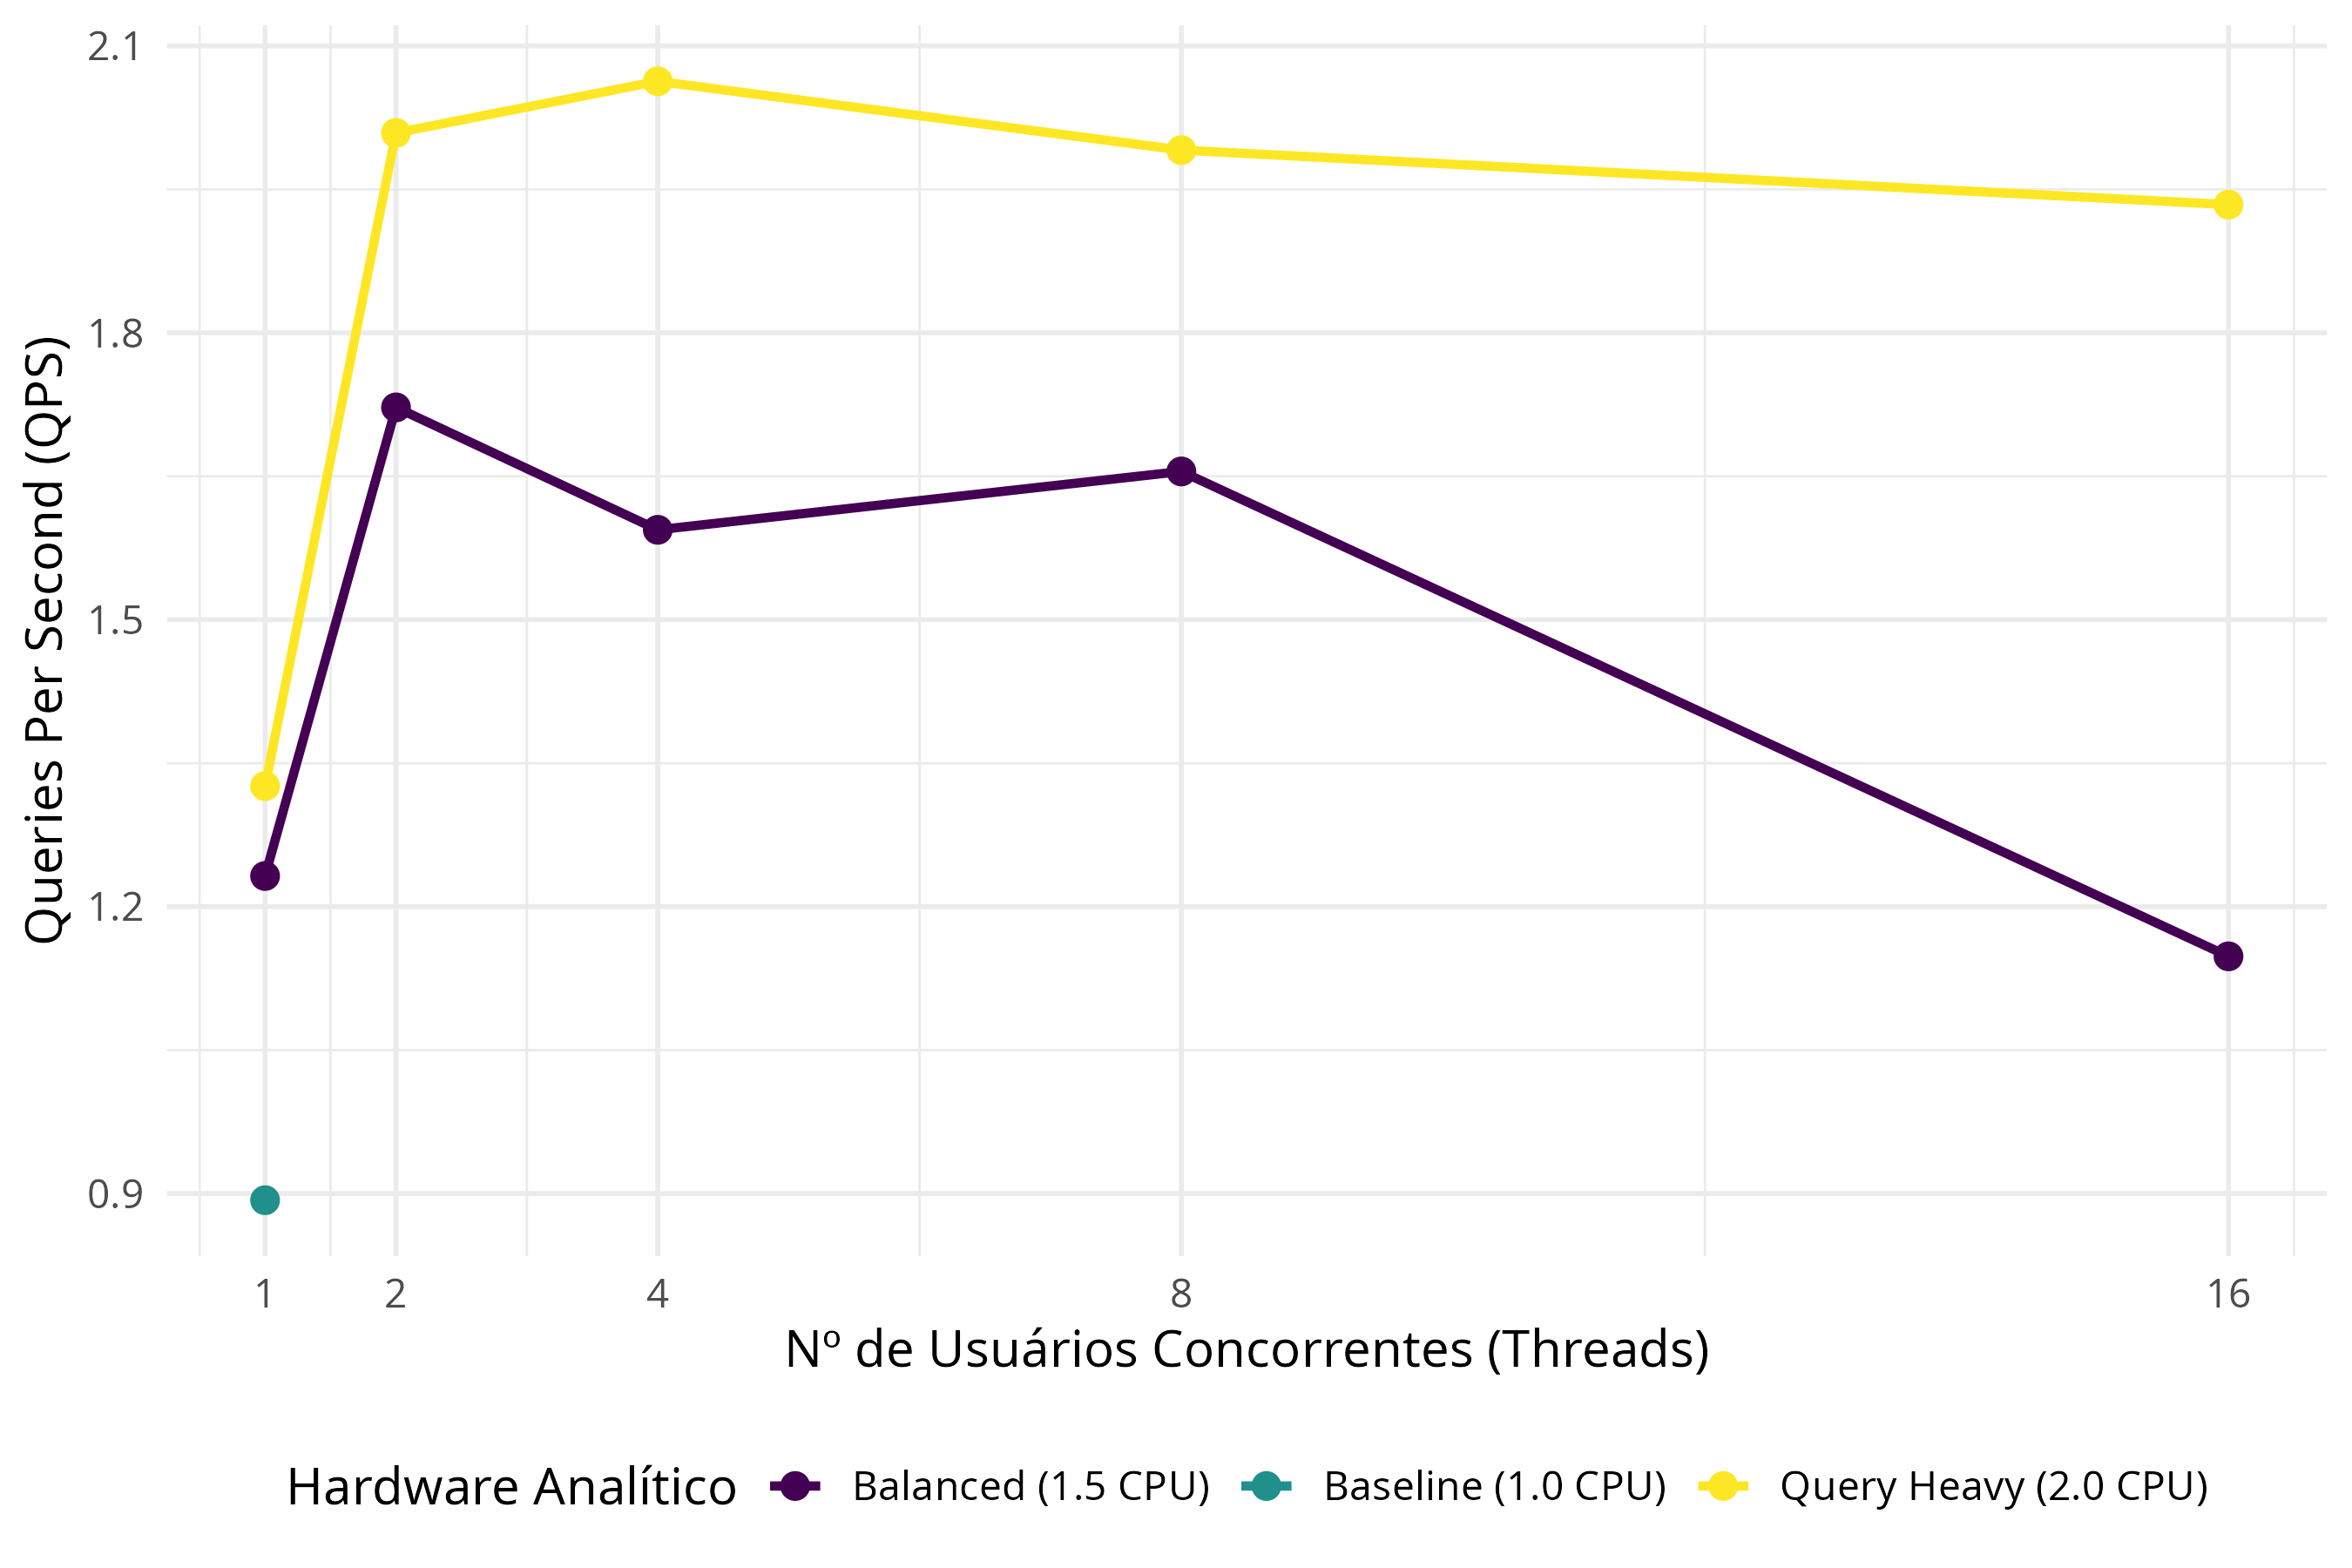
\includegraphics[width=0.47\linewidth]{fig_qps_saturation.png} &
    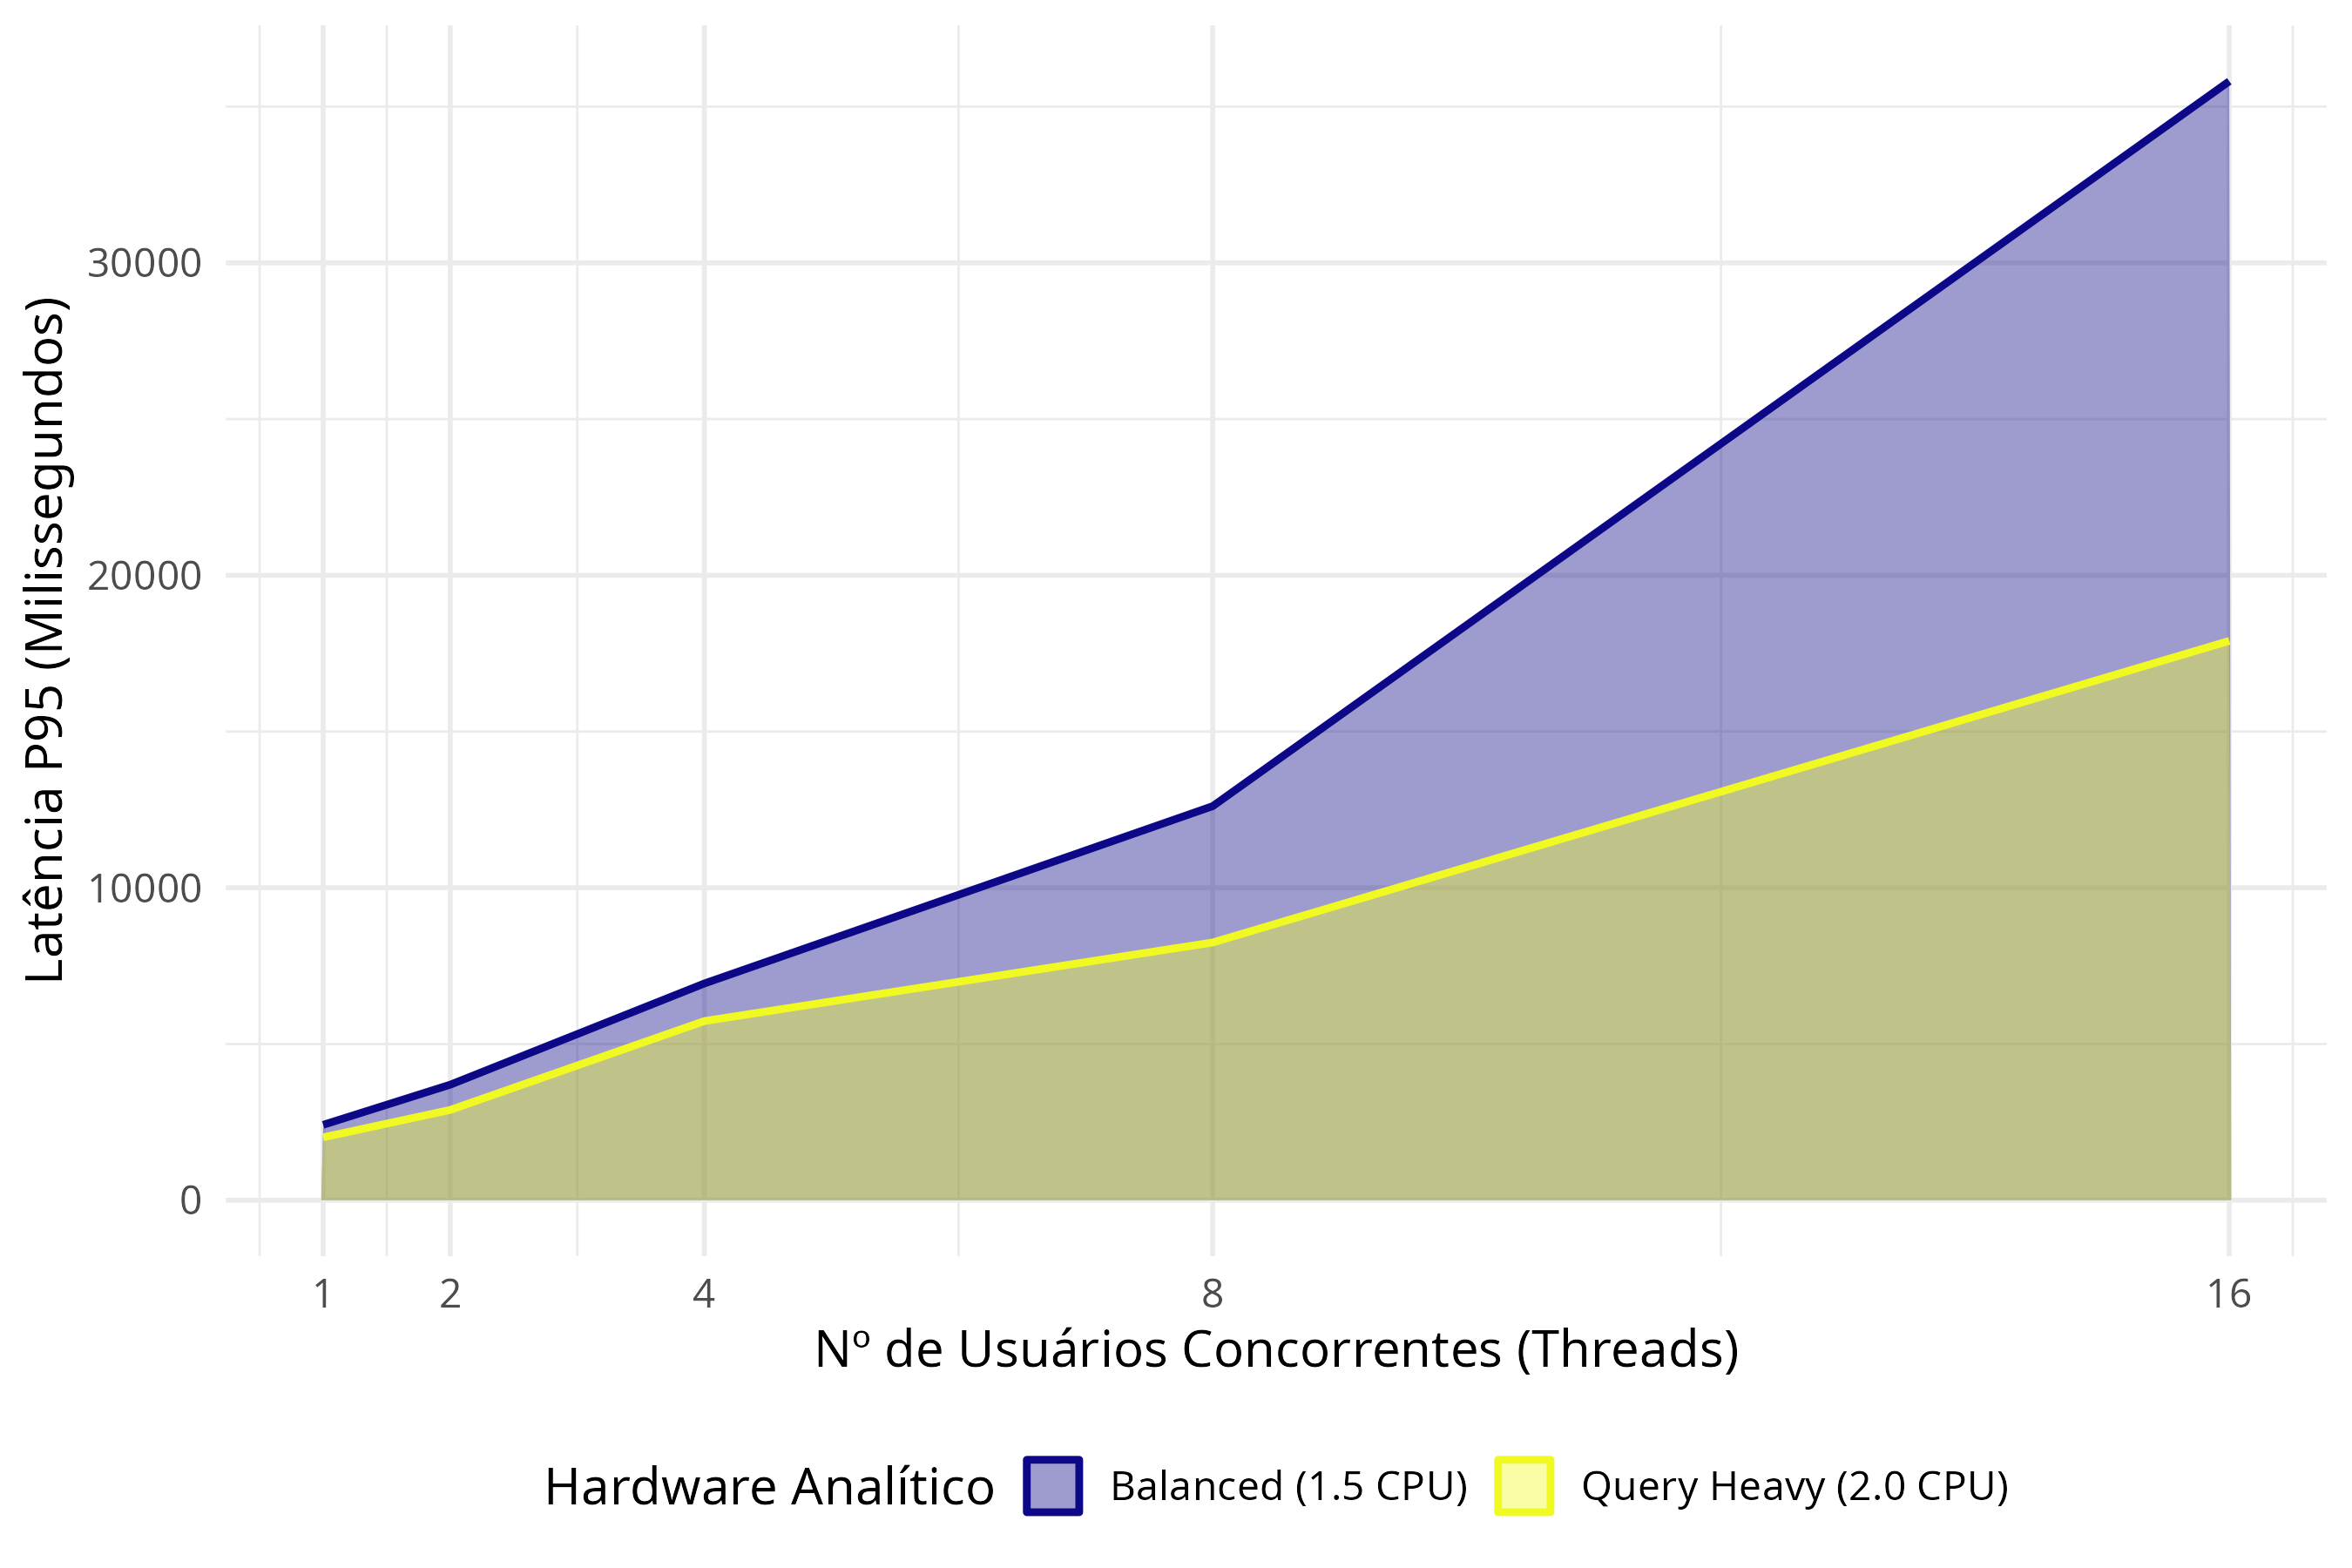
\includegraphics[width=0.47\linewidth]{fig_p95_latency.png} \\
    {\fontsize{13}{16}\selectfont (a) Vazão analítica (QPS) sob estresse} &
    {\fontsize{13}{16}\selectfont (b) Latência P95 por concorrência} \\[0.18cm]
    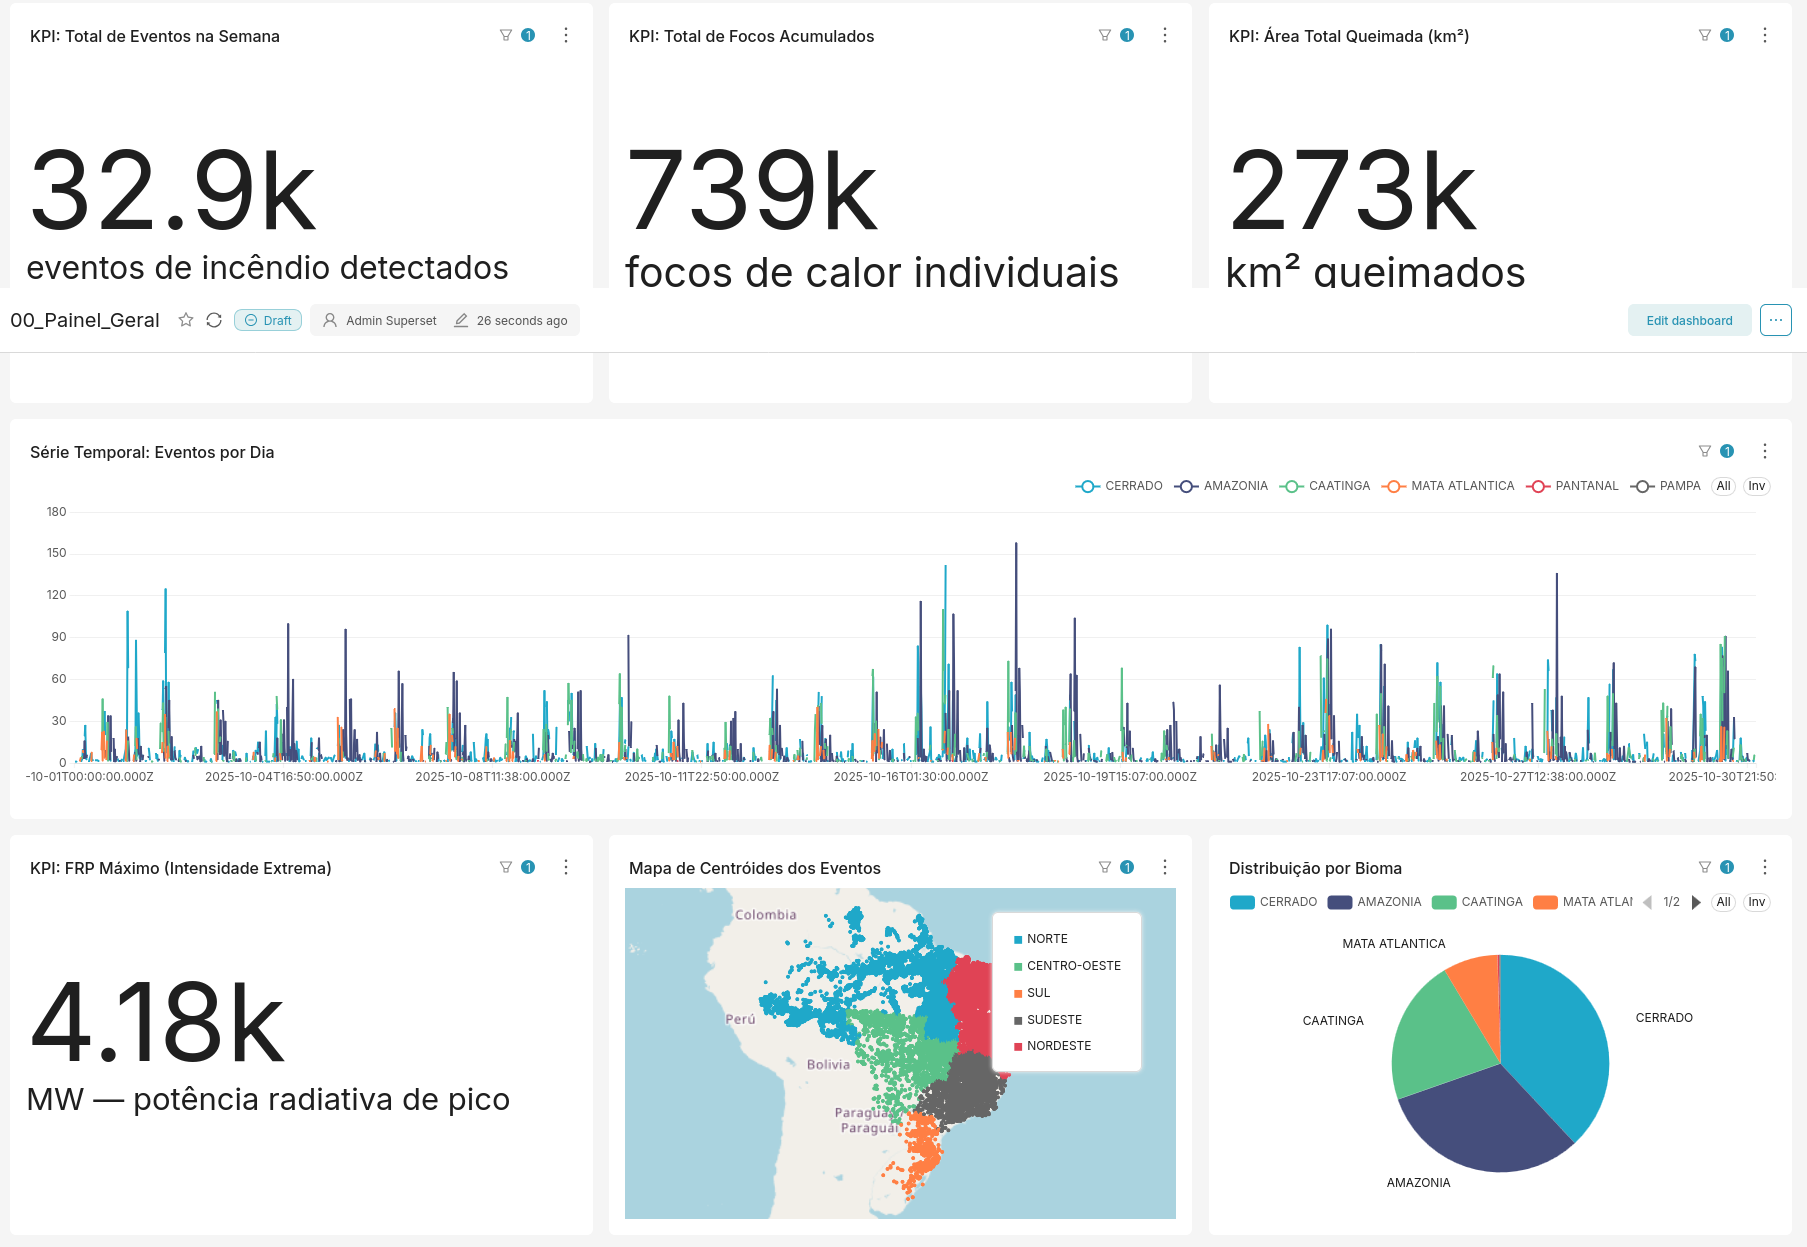
\includegraphics[width=0.47\linewidth]{fig_dashboard_superset.png} &
    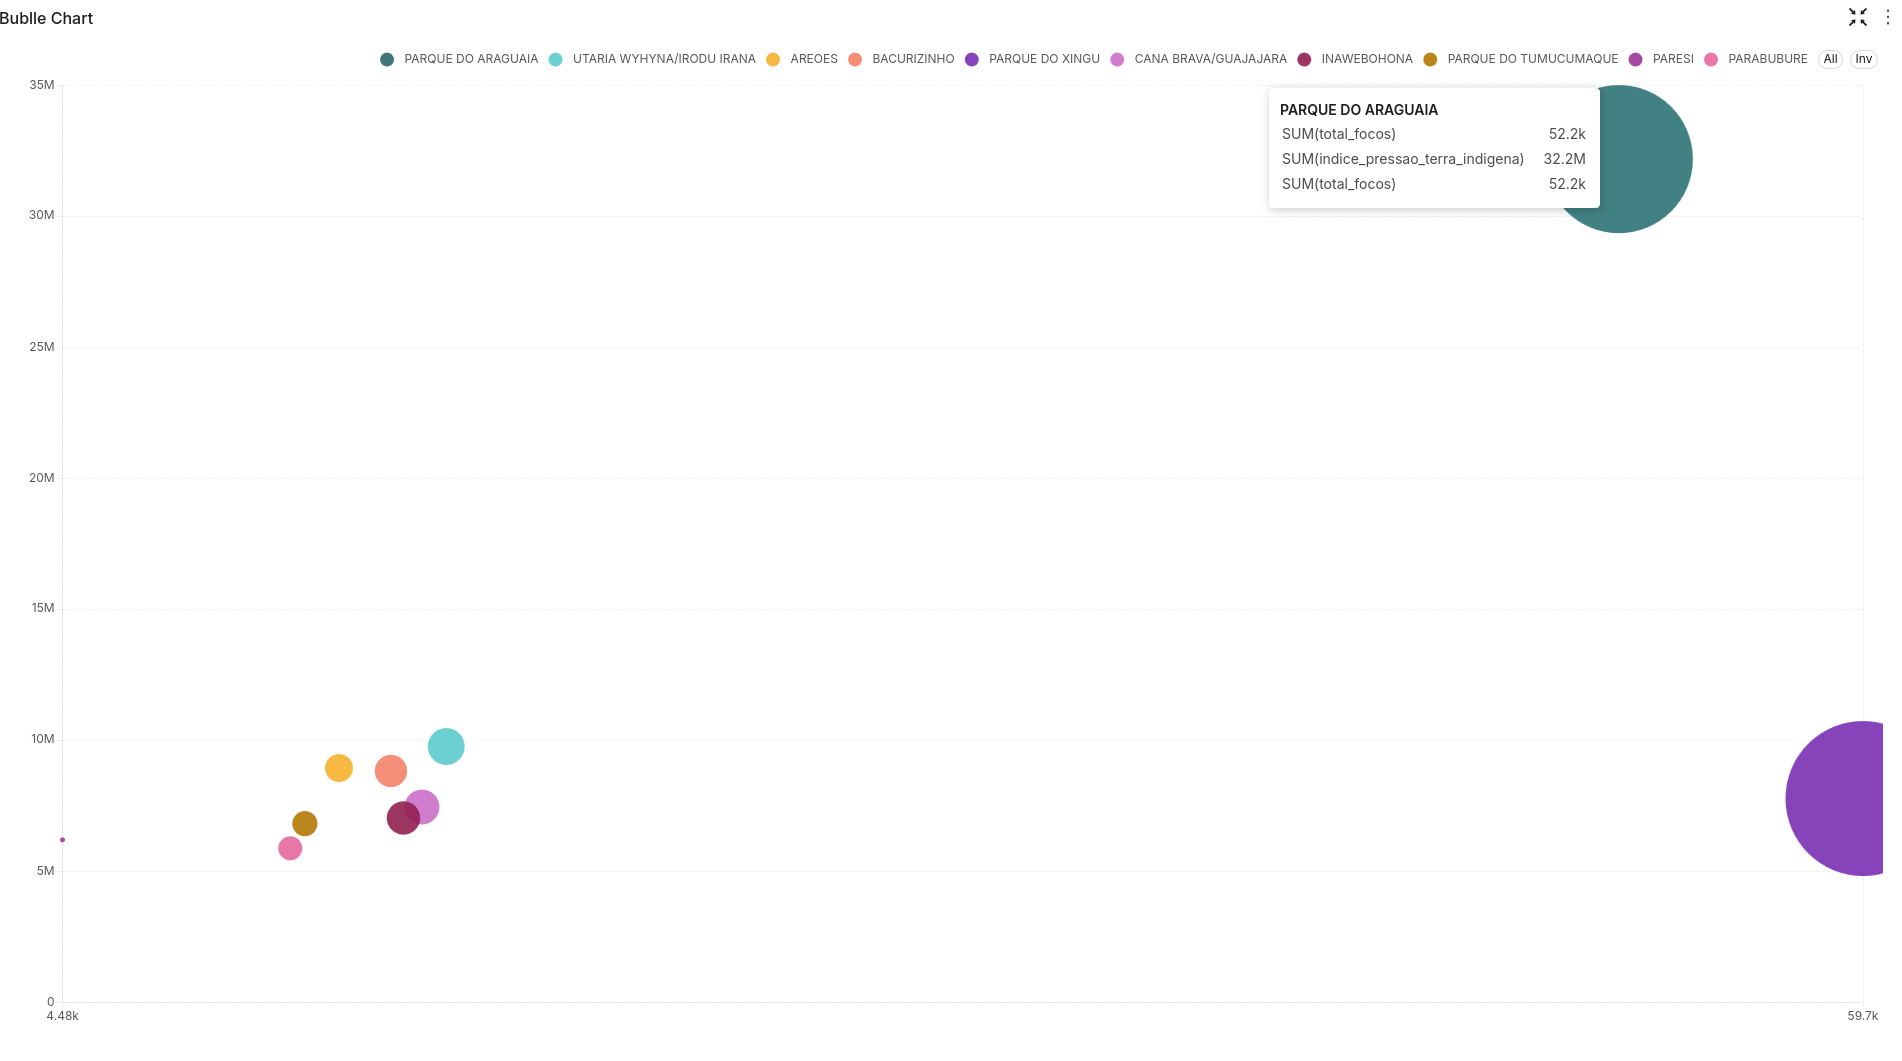
\includegraphics[width=0.47\linewidth]{fig_pressao_indigena.png} \\
    {\fontsize{13}{16}\selectfont (c) Painel tático geral (\textbf{\textit{Superset}})} &
    {\fontsize{13}{16}\selectfont (d) Pressão sobre Terras Indígenas (\textbf{\textit{Bubble Chart}})} \\
\end{tabular}
\vspace{0.08cm}
\captionof{figure}{Evidências empíricas de desempenho analítico e inteligência tática no Brasil.}
\label{fig:grid_resultados}
\end{center}

Na camada de visualização, os painéis operacionais no \textbf{\textit{Apache Superset}} consolidam o fluxo analítico contínuo para subsidiar a tomada de decisão das equipes de emergência e Defesa Civil. A interface gerencial centraliza a contagem de focos ativos e a severidade térmica (FRP), oferecendo filtros dinâmicos por bioma e horizonte temporal para triagens rápidas (Fig. 3c). 

Para além da contagem volumétrica bruta de detecções, a plataforma calcula a pressão contínua exercida sobre áreas protegidas, ponderando a potência radiativa do fogo, o risco meteorológico e o decaimento com a distância: \textbf{\textit{($\boldsymbol{I_{\text{pressão}} = \frac{\text{FRP} \times (1 + \text{risco})}{\max(d_{\text{km}},\, 0{,}1)}}$)}}. A análise sobre os dados de 2025 sugere a existência de um padrão cíclico sazonal de vulnerabilidade térmica, no qual a Terra Indígena Parque do Araguaia (TO) despontou no primeiro lugar em exposição acumulada durante o período de estiagem (Fig. 3d). Essa leitura antecipatória justifica-se pela dinâmica recorrente de avanço do fogo sobre territórios tradicionais, corroborada na prática pelo incêndio de grandes proporções que destruiu dezenas de moradias na Aldeia Canoanã em Formoso do Araguaia (G1 TOCANTINS, 2026).
